\section{Dynamic Proxy}

\subsection{Java's Dynamic Proxy}

\subsubsection{What Is a Proxy?}

The homonym design pattern defines a proxy as an:

\begin{itemize}
	\item object providing a surrogate/placeholder for another object
	\item to control and manipulate the accesses to it
\end{itemize}

Few examples

\begin{itemize}
	\item local representation of remote objects;
	\item delay of expensive operations;
	\item access protection for secure objects.
\end{itemize}

\subsubsection{What Is a Dyniamic Proxy?}

A dynamic proxy class is a class implementing a \textbf{list of interfaces} such that the invocation of a method beloging to one of these interfaces on one of its instances is \textbf{seamleassly dispatched} to another object implementing such interface and bound to the dynamic proxy object.

A dynamic proxy class can be used to create a type-safe proxy object for a set of objects determined by the implemented interfaces \textbf{without} both \textbf{explicit coding} and \textbf{static pre generation} of the proxy class as happens with several compile-time tools.

Dynamic proxy classes are useful to applications or libraries that need to provide type-safe reflective dispatch of invocations on objects whose interface is available

java.lang.reflect.InvocationHandler

\subsubsection{java.lang.reflect.InvocationHandler}

Each proxy instance has an associated invocation handler.

When a method is invoked on a proxy instance

\begin{itemize}
	\item the method invocation is dispatched to the invoke() method of its invocation handler
\end{itemize}

\begin{center}
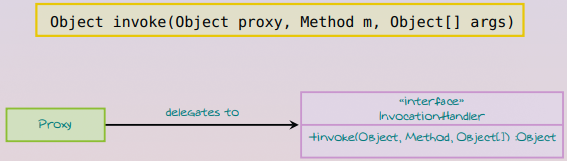
\includegraphics[scale=0.7]{10-invocation-handler}
\end{center}

\subsubsection{java.lang.reflect.Proxy}

Proxy

\begin{itemize}
	\item  provides static methods for creating dynamic proxy classes and instances, and
	\item  it also is the superclass of all dynamic proxy classes created by these methods
\end{itemize}

\begin{lstlisting}[language=Java]
public final class Proxy extends Object implements Serializable {
	protected InvocationHandler h;
	protected Proxy(InvocationHandler h) { ... }
	public static InvocationHandler getInvocationHandler(Object proxy) { ... }
	public static Class<?> getProxyClass(ClassLoader l, Class<?>... interfaces) { ... }
	public static boolean isProxyClass(Class<?> cl) { ... }
	public static Object newProxyInstance(ClassLoader loader, Class<?>[] interfaces, InvocationHandler h ) { ... }
}
\end{lstlisting}

Basically, Proxy enables the meta-object approach in Java

\subsubsection{How Java Creates a Proxy}

\begin{center}
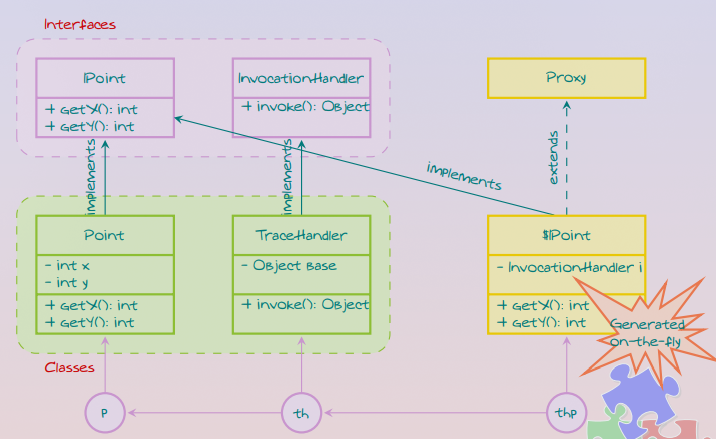
\includegraphics[scale=0.4]{11-create-a-proxy}
\end{center}

\subsubsection{Example: To Trace the Method Calls}

\begin{lstlisting}[language=Java]
import java.lang.reflect.*;
public class TraceHandler implements InvocationHandler {
	private Object baseObject;
	public TraceHandler(Object base) { baseObject = base; }
	public Object invoke(Object proxy, Method m, Object[] args) {
	try {
		System.out.println("before " + m.getName());
		Object result = m.invoke(baseObject, args);
		System.out.println("after " + m.getName());
		return result;
	} catch (Exception e) {
		e.printStackTrace(); 
		return null;
	}
}
public String toString() { return "th :- "+this.baseObject; }
}
\end{lstlisting}

\begin{lstlisting}[language=Java]
jshell> IPoint p1 = new Point(10,20);
p1 ==> p :- (10, 20)
jshell> IPoint th_p1 = (IPoint) Proxy.newProxyInstance(
p1.getClass().getClassLoader(), p1.getClass().getInterfaces(), new TraceHandler(p1));
before toString
after toString
th_p1 ==> p :- (10, 20)
jshell> p1.getX(); /* standard call */
$10 ==> 10
jshell> th_p1.getX(); /* traced call */
before getX
after getX
$11 ==> 10
\end{lstlisting}

\subsubsection{Example: Invariant Checking and Proxy Chaining}

\begin{lstlisting}[language=Java]
import java.lang.reflect.*;

public class InvariantHandler implements InvocationHandler {
	private Object target;
	private Method invariant;
	public InvariantHandler(Object target) {
		this.target = target;
		try {
			invariant = target.getClass().getMethod("invariant", new Class<?>[]{});
			if (!invariant.getReturnType().equals(boolean.class)) invariant = null;
		} 
		catch (NoSuchMethodException ex) { 
			invariant = null; }
		}
		
public Object invoke(Object proxy, Method method, Object[] args) throws Throwable {
	this.invokeInvariant(method);
	Object retvalue = method.invoke(this.target, args);
	this.invokeInvariant(method);
	return retvalue;
}

private void invokeInvariant(Method method) {
	if ((this.invariant == null) || (method.equals(this.invariant))) return;
	try {
		Boolean passed = (Boolean) invariant.invoke(target, new Object[]{});
		if (!passed.booleanValue()) throw new RuntimeException();
	} catch (Exception e) {
		System.out.println("Failed invariant check!!!"); 
	}
}
public String toString() {return "ih :- "+this.target; }
}
\end{lstlisting}

\subsubsection{Example: Invariant Checking and Proxy Chaining (Cont'd)}

\begin{lstlisting}[language=Java]
jshell> InvariantHandler ih = new InvariantHandler(new Point(0, 7));
ih ==> ih :- p :- (0, 7)
jshell> IPoint invariantCheckedPoint =
(IPoint)Proxy.newProxyInstance(
Point.class.getClassLoader(),
new Class[]{ IPoint.class }, ih);
invariantCheckedPoint ==> p :- (0, 7)
jshell> TraceHandler th = new TraceHandler(invariantCheckedPoint);
th ==> th :- p :- (0, 7)
jshell> IPoint tracedInvariantCheckedPoint =
(IPoint)Proxy.newProxyInstance(
Point.class.getClassLoader(),
new Class[] { IPoint.class }, th);
before toString
after toString
tracedInvariantCheckedPoint ==> p :- (0, 7)
jshell> tracedInvariantCheckedPoint.setX(25)
before setX
after setX
jshell> tracedInvariantCheckedPoint.setY(-7)
before setY
Failed invariant check!!!
after setY
\end{lstlisting}

\subsubsection{Example: Invariant Checking and Proxy Chaining (Cont'd)}

\begin{center}
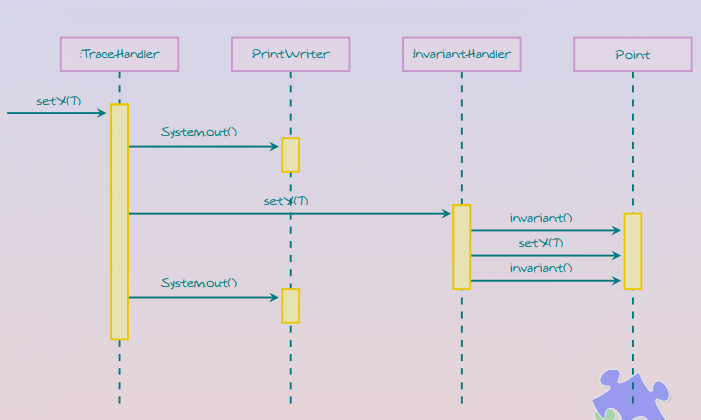
\includegraphics[scale=0.4]{12-proxy-chaining}
\end{center}


